\documentclass[12pt]{article}
\usepackage{url}
\usepackage{arxiv}
\usepackage[utf8]{inputenc} % allow utf-8 input
\usepackage[T1]{fontenc}    % use 8-bit T1 fonts
\usepackage[pdftex]{hyperref}       % hyperlinks
\usepackage{mathptmx}
\usepackage{fullpage}
\usepackage{array, booktabs}       % professional-quality tables
\usepackage{amsfonts}       % blackboard math symbols
\usepackage{nicefrac}       % compact symbols for 1/2, etc.
\usepackage{microtype}      % microtypography
\usepackage{lipsum}
\usepackage{graphicx}
\usepackage{xcolor}
\usepackage{placeins}
\usepackage{amsmath}
\usepackage{tcolorbox}
\usepackage{xcolor}
\usepackage{url}
\usepackage{array}
\usepackage{relsize}
\usepackage{minted}
\usepackage[hyperref=true,
            url=true,
            isbn=false,
            backref=true,
            style=numeric,
            maxcitenames=3,
            maxbibnames=100,
            block=none]{biblatex}
\addbibresource{./refs/refs.bib}
\newcolumntype{R}{>{\raggedleft\arraybackslash}m{3cm}}
\textwidth=8cm
\parindent=0pt
\hypersetup{colorlinks=true,linkcolor=blue, filecolor=magenta, urlcolor=cyan}
\definecolor{offwhite}{HTML}{F7F6F6}
\makeatletter
\g@addto@macro{\UrlBreaks}{\UrlOrds}
\makeatother

\title{The SportsDataverse: An Open Sports Data Initiative}

\author{
%  Saiem Gilani \\
%   Lead Engineer\\
%   SportsDataverse.org\\
%   \texttt{saiem.gilani@gmail.com} \\
}

\begin{document}
 \maketitle

\section{Introduction}
One of the animating forces at the core of a thriving research community is the availability of open data. This streamlines the process to provide standardized datasets and lays the groundwork for reproducible research and creates more accessible opportunities for research and development among the broader data community.  Taking note of the sports analytics papers of the last several years and their impact on the research community, one stands out among all others, \emph{nflWAR: A Reproducible Method for Offensive Player Evaluation in Football}~\cite{yurko_venturahorowitz_2019}. This paper was accompanied with the release of the \texttt{nflscrapR} package, which allowed for the reproducibility of the results of the paper. The package was wildly popular, but there was pressure to keep the package and data maintained long after the paper was demonstrated to be reproducible, and eventually the package was replaced with the \href{https://www.nflfastR.com}{\texttt{nflfastR}} package~\cite{Carl_Baldwin_2020}. The combined efforts of Sebastian Carl and the rest of the nflverse team have set a golden standard for operating a set of open-source sports data packages worthy of praise and emulation. 

\section{The SportsDataverse Initiative}
The \href{https://sportsdataverse.org}{SportsDataverse} is a broader concept to produce a more cohesive set of open-source sports data packages with emphasis on improving testing standards and creating search-able documentation websites. The aim is to have these resources serve as steadfast public utilities \textbf{maintained by the community of developers} for research and development. The intention is for projects to build on top of these packages to prototype ideas and, if desired and deemed appropriate, merge relevant portions of their idea to the data processing pipeline and packages.

The SportsDataverse developer group has created a collection of software packages for sports data with modules written in Python, R, and Node.js. Collectively, the SportsDataverse packages cover 18 sports leagues worth of data, including 11+ men's sports and 7+ women's sports with plans for expansion. 

Several of the packages written are directly modeled on the data engineering efforts of the \texttt{nflfastR} team, including \texttt{cfbfastR(py)}\cite{sgetal2021cfbfastr}\cite{gilani_cfbfastRpy_2021}, \texttt{hoopR(py)}\cite{gilani_hoopRpy_2021}\cite{gilani_cfbfastRpy_2021}, and \texttt{wehoop(py)}. These packages allow for the loading of play-by-play and box score data for 16+ seasons of data for NBA, WNBA, men's and women's college basketball, and college football with parallel processing and progress updates. This saves the user countless hours of setting up a web scrape, setting up a cron job to schedule automated data extracts and allows them to spend more time building their project rather than building the data infrastructure and pipeline from scratch.  

\section{Data and Programming Language Considerations}
The programming languages of Python, R and Node.js were chosen for their widespread usage among the data science, sports analytics, and application development communities. 
Though there is no current intention to extend to more languages, the data repositories made available through the use of the existing packages can be accessed via your preferred language of choice as painlessly as downloading any file from a URL would be. Most data are available in multiple formats of \texttt{CSV}, \texttt{Rds}, \texttt{JSON} or \texttt{Parquet} for ease of inter-language use. Among the goals of the SportsDataverse is to flatten the learning curve the average user has to go through to get access to high quality open-source sports data and analytics. While the utility building and function packaging portion of the project is a "work in progress", we have successfully created an exceptional collection of open-source sports data repositories on GitHub. For example, from the packages I directly contribute to, we have generated \textbf{over 250 gigabytes of data} in the aforementioned formats for use in loading and reference across the SportsDataverse. 

\section{R Packages}
While there are a number of R packages within the SportsDataverse, for the sake of brevity, I will briefly discuss three in this paper -- \texttt{cfbfastR} for college football, \texttt{hoopR} for NBA and men's college basketball, and \texttt{wehoop} for WNBA and women's college basketball coverage. Each package has the ability to load 16+ seasons of play-by-play data for each sport covered, from which users can then create their own processing pipeline for their own analyses. Additionally, each package also allows for access to live game data through access to ESPN's content delivery networks (CDN) and application programming interfaces (API). 

\subsection{Package Installations}
The packages listed above are being prepared for submission to CRAN (the Comprehensive R Archive Network) and thus must be installed from GitHub. I prefer the \texttt{pacman} installation method as follows:
\usemintedstyle{friendly}
\begin{minted}
[
baselinestretch=1.2,
bgcolor=offwhite,
fontsize=\footnotesize
]
{R}
if (!requireNamespace('pacman', quietly = TRUE)){
  install.packages('pacman')
}
pacman::p_load_current_gh("saiemgilani/cfbfastR", "saiemgilani/hoopR", "saiemgilani/wehoop")

\end{minted}

\subsection{cfbfastR}

\subsubsection{How it Started -- \texttt{cfbscrapR}}
The initial origin of this package was to provide the collegiate equivalent of the \texttt{nflscrapR} package, producing expected points metrics and win probability models. This was accomplished successfully in the \href{https://www.github.com/saiemgilani/cfbscrapR}{\texttt{cfbscrapR}}-era\cite{subbiahgilanifleming_2020} of the package. While \texttt{cfbfastR} is the successor of the \texttt{cfbscrapR} package, the packages are largely the same, with a handful of extra features. 
\subsubsection{College Football Data API}
\texttt{cfbfastR} is the unofficial R client for the \href{CollegeFootballData.com}{https://www.CollegeFootballData.com} API, a resource provided by Bill Radjewski, which allows programmatic access a database with a number of views for users to query with a free API key. 

\subsection{hoopR}
\usemintedstyle{friendly}
\begin{minted}
[
baselinestretch=1.2,
bgcolor=offwhite,
fontsize=\footnotesize
]
{R}

\end{minted}


\subsection{wehoop}
\usemintedstyle{friendly}
\begin{minted}
[
baselinestretch=1.2,
bgcolor=offwhite,
fontsize=\footnotesize
]
{R}
pacman::p_load_current_gh("saiemgilani/wehoop")

\end{minted}
\subsubsection{WNBA full play-by-play seasons (2002-2021) ~ 1-2 minutes}
\usemintedstyle{friendly}
\begin{minted}
[
baselinestretch=1.2,
bgcolor=offwhite,
fontsize=\footnotesize
]
{R}
future::plan("multisession")
tictoc::tic()
progressr::with_progress({
  wnba_pbp <- wehoop::load_wnba_pbp(2002:2021)
})
tictoc::toc()
## 12.01 sec elapsed
glue::glue("{nrow(wnba_pbp)} rows of WNBA play-by-play data from {length(unique(wnba_pbp$game_id))} games.")
## 1782985 rows of WNBA play-by-play data from 4674 games.
# Rows: 1,782,985
# Columns: 42
#$ shooting_play             <lgl> FALSE, FALSE, TRUE, FALSE, TRUE, ~
#$ sequence_number           <chr> "1", "2", "3", "4", "5", "6", "7"~
#$ period_display_value      <chr> "1st Quarter", "1st Quarter", "1s~
#$ period_number             <int> 1, 1, 1, 1, 1, 1, 1, 1, 1, 1, 1, ~
#$ home_score                <int> 0, 0, 0, 0, 0, 0, 0, 0, 0, 0, 0, ~
#$ coordinate_x              <int> 0, 0, 35, 0, 40, 0, 0, 25, 0, 0, ~
#$ coordinate_y              <int> 0, 0, 11, 0, 5, 0, 0, 0, 0, 0, 0,~
#$ scoring_play              <lgl> FALSE, FALSE, FALSE, FALSE, FALSE~
#$ clock_display_value       <chr> "20:00", "20:00", "19:34", "19:31~
#$ team_id                   <chr> NA, "6", "6", "9", "9", "6", "6",~
#$ type_id                   <chr> "411", "615", "20558", "587", "20~
#$ type_text                 <chr> "Start Period", "Jumpball", "Jump~
#$ away_score                <int> 0, 0, 0, 0, 0, 0, 0, 2, 2, 2, 3, ~
#$ id                        <dbl> 22052500600000, 22052500600001, 2~
#$ text                      <chr> "Start of the 1st Half.", "Jumpba~
#$ score_value               <int> 0, 0, 0, 0, 0, 0, 0, 2, 0, 0, 1, ~
#$ participants_0_athlete_id <chr> NA, "18", "7", "21", "18", "6", "~
#$ participants_1_athlete_id <chr> NA, "6", NA, NA, NA, NA, "6", "20~
#$ participants_2_athlete_id <chr> NA, "9", NA, NA, NA, NA, NA, NA, ~
#$ type_abbreviation         <lgl> NA, NA, NA, NA, NA, NA, NA, NA, N~
#$ season                    <int> 2002, 2002, 2002, 2002, 2002, 200~
#$ season_type               <int> 2, 2, 2, 2, 2, 2, 2, 2, 2, 2, 2, ~
#$ away_team_id              <int> 9, 9, 9, 9, 9, 9, 9, 9, 9, 9, 9, ~
#$ away_team_name            <chr> "New York", "New York", "New York~
#$ away_team_mascot          <chr> "Liberty", "Liberty", "Liberty", ~
#$ away_team_abbrev          <chr> "NYL", "NYL", "NYL", "NYL", "NYL"~
#$ away_team_name_alt        <chr> "New York", "New York", "New York~
#$ home_team_id              <int> 6, 6, 6, 6, 6, 6, 6, 6, 6, 6, 6, ~
#$ home_team_name            <chr> "Los Angeles", "Los Angeles", "Lo~
#$ home_team_mascot          <chr> "Sparks", "Sparks", "Sparks", "Sp~
#$ home_team_abbrev          <chr> "LOS", "LOS", "LOS", "LOS", "LOS"~
#$ home_team_name_alt        <chr> "Los Angeles", "Los Angeles", "Lo~
#$ home_team_spread          <dbl> 2.5, 2.5, 2.5, 2.5, 2.5, 2.5, 2.5~
#$ game_spread               <dbl> 2.5, 2.5, 2.5, 2.5, 2.5, 2.5, 2.5~
#$ home_favorite             <lgl> TRUE, TRUE, TRUE, TRUE, TRUE, TRU~
#$ clock_minutes             <chr> "20", "20", "19", "19", "19", "19~
#$ clock_seconds             <chr> "00", "00", "34", "31", "21", "19~
#$ half                      <chr> "1", "1", "1", "1", "1", "1", "1"~
#$ lag_half                  <chr> NA, "1", "1", "1", "1", "1", "1",~
#$ lead_half                 <chr> "1", "1", "1", "1", "1", "1", "1"~
#$ game_play_number          <int> 1, 2, 3, 4, 5, 6, 7, 8, 9, 10, 11~
#$ game_id                   <int> 220525006, 220525006, 220525006, ~
\end{minted}

\subsubsection{WNBA full team box score seasons (2002-2021) ~ 5-30 seconds}
\usemintedstyle{friendly}
\begin{minted}
[
baselinestretch=1.2,
bgcolor=offwhite,
fontsize=\footnotesize
]
{R}
future::plan("multisession")
tictoc::tic()
progressr::with_progress({
  wnba_team_box <- wehoop::load_wnba_team_box(2002:2021)
})
tictoc::toc()
## 8.06 sec elapsed 
glue::glue("{nrow(wnba_team_box)} rows of WNBA team boxscore data from {length(unique(wnba_team_box#$game_id))} games.")
## 8624 rows of WNBA team boxscore data from 4312 games.
\end{minted}


\subsubsection{WNBA full player box score seasons (2002-2021) ~ 5-30 seconds}
\usemintedstyle{friendly}
\begin{minted}
[
baselinestretch=1.2,
bgcolor=offwhite,
fontsize=\footnotesize
]
{R}
future::plan("multisession")
tictoc::tic()
progressr::with_progress({
  wnba_player_box <- wehoop::load_wnba_player_box(2002:2021)
})
tictoc::toc()
## 8.06 sec elapsed 
glue::glue("{nrow(wnba_player_box)} rows of WNBA player boxscore data from {length(unique(wnba_player_box#$game_id))} games.")
## 8624 rows of WNBA player boxscore data from 4312 games.
\end{minted}


The first phase of the initiative is to broaden the number of sports the packages covered by the packages through existing data sources, to improve the quality of the existing packages, and to recruit existing open-source sports data packages and their developers to the organization.


The end goal of the initiative would allow the interested to get started in sports analytics with a command as simple as: 
\usemintedstyle{friendly}
\begin{minted}
[
baselinestretch=1.2,
bgcolor=offwhite,
fontsize=\footnotesize
]
{R}
# Python
pip install sportsdataverse
# R
install.packages(sporstdataverse)
# Node.js
yarn add sportsdataverse
\end{minted}
\section{Python Packages to Date}
These are the packages that have agreed to join us from the Python community:
\begin{table}[!htbp]
\centering
\renewcommand{\arraystretch}{1.3}
\begin{tabular}{>{\raggedright}m{1.0in} >{\raggedright}m{2.2in} >{\centering}m{0.8in} >{\raggedright\arraybackslash}m{2.0in}}
\toprule
\multicolumn{4}{c}{\textbf{Python Packages in the SportsDataverse}} \\
\textbf{Package} & \textbf{Sports Leagues} & \textbf{Repository} & \textbf{Author(s)} \\ 
 \midrule
    cfbfastR-py & College Football & \href{https://github.com/saiemgilani/cfbfastR-py/}{GitHub} - \href{https://cfbfastR-py.sportsdataverse.org/}{Docs} & Saiem Gilani\\
    hoopR-py & NBA and Men's College Basketball & \href{https://github.com/saiemgilani/hoopR-py/}{GitHub} - \href{https://hoopR-py.sportsdataverse.org}{Docs} & Saiem Gilani \\
    recruitR-py & Men's College Sports Recruiting & \href{https://github.com/saiemgilani/recruitR-py/}{GitHub} - \href{https://saiemgilani.github.io/recruitR/}{Docs} & Saiem Gilani, Bud Davis \\
    wehoop-py & WNBA and Women's College Basketball & \href{https://github.com/saiemgilani/wehoop-py}{GitHub} - \href{https://wehoop-py.sportsdataverse.org}{Docs} & Saiem Gilani \\
    powerplay-py & NHL & \href{https://github.com/saiemgilani/powerplay-py}{GitHub} - \href{https://saiemgilani.github.io/powerplay}{Docs} & Saiem Gilani \\
\bottomrule
\end{tabular}
\vspace{5pt}
\caption{Python packages contributed to the SportsDataverse}
\label{tbl:sdvpy}
\vspace{-5mm}
\end{table}
\newline


\subsection{R Packages to Date}
These are the packages that have agreed to join us from the R community:
\begin{table}[!htbp]
\centering
\renewcommand{\arraystretch}{1.3}
\begin{tabular}{>{\raggedright}m{1.0in} >{\raggedright}m{2.2in} >{\centering}m{0.8in} >{\raggedright\arraybackslash}m{2.0in}}
\toprule
\multicolumn{4}{c}{\textbf{R Packages in the SportsDataverse}} \\
\textbf{Package} & \textbf{Sports Leagues} & \textbf{Repository} & \textbf{Author(s)} \\ 
 \midrule
    cfbfastR & College Football & \href{https://github.com/saiemgilani/cfbfastR/}{GitHub} - \href{https://saiemgilani.github.io/cfbfastR/}{Docs} & Saiem Gilani, Akshay Easwaran, Jared Lee, Eric Hess \\
    gamezoneR  & Men's and Women's College Basketball & \href{https://github.com/jacklich10/gamezoneR/}{GitHub} - \href{https://jacklich10.github.io/gamezoneR/}{Docs} & Jack Lichtenstein \\
    hoopR & NBA and Men's College Basketball & \href{https://github.com/saiemgilani/hoopR/}{GitHub} - \href{https://hoopR.sportsdataverse.org}{Docs} & Saiem Gilani \\
    puntr & NFL and College Football & \href{https://github.com/Puntalytics/puntr}{GitHub} - \href{https://puntalytics.github.io/puntr/}{Docs} & Dennis Brookner and Raphael LadenGuindon \\
    recruitR & Men's College Sports Recruiting & \href{https://github.com/saiemgilani/recruitR/}{GitHub} - \href{https://saiemgilani.github.io/recruitR/}{Docs} & Saiem Gilani \\
    wehoop & WNBA and Women's College Basketball & \href{https://github.com/saiemgilani/wehoop}{GitHub} - \href{https://wehoop.sportsdataverse.org}{Docs} & Saiem Gilani and Geoff Hutchinson \\
    worldfootballR & EPL, La Liga, Bundesliga, Serie A, Ligue 1, RFPL & \href{https://github.com/JaseZiv/worldfootballR}{GitHub} - \href{https://jaseziv.github.io/worldfootballR}{Docs} & Jason Zivkovic \\
    powerplay & NHL & \href{https://github.com/saiemgilani/powerplay}{GitHub} - \href{https://saiemgilani.github.io/powerplay}{Docs} & Saiem Gilani \\
    hockeyR & NHL & \href{https://github.com/danmorse314/hockeyR/}{GitHub} - \href{https://hockeyr.netlify.app/}{Docs} & Dan Morse \\
    baseballr & NHL & \href{https://github.com/BillPetti/baseballr/}{GitHub} - \href{https://BillPetti.github.io/baseballr}{Docs} & Bill Petti \\
\bottomrule 
\end{tabular}
\vspace{5pt}
\caption{R Packages contributed to the SportsDataverse}
\label{tbl:sdvr}
\vspace{-5mm}
\end{table}


\subsection{Node.js Packages to Date}
These are the packages that have agreed to join us from the Node.js community:

\begin{table}[!htbp]
\centering
\renewcommand{\arraystretch}{1.3}
\begin{tabular}{>{\raggedright}m{1.0in} >{\raggedright}m{2.2in} >{\centering}m{0.8in} >{\raggedright\arraybackslash}m{2.0in}}
\toprule
\multicolumn{4}{c}{\textbf{Node.js Packages in the SportsDataverse}} \\
\textbf{Package} & \textbf{Sports Leagues} & \textbf{Repository} & \textbf{Author(s)} \\ 
 \midrule
    sportsdataverse & College Football & \href{https://github.com/saiemgilani/sportsdataverse/}{GitHub} - \href{https://saiemgilani.github.io/sportsdataverse}{Docs} & Saiem Gilani\\
    @sportsdataverse/nhl & NHL & \href{https://github.com/saiemgilani/sportsdataverse-nhl/}{GitHub} & Saiem Gilani \\
    nfl-nerd & Men's College SportsRecruiting & \href{https://github.com/nntrn/nfl-nerd/}{GitHub} & Annie Tran \\
\end{tabular}
\vspace{5pt}
\caption{Node.js modules contributed to the SportsDataverse}
\label{tbl:sdvjs}
\vspace{-5mm}
\end{table}


%\begin{table}[!htbp]
%\centering
%\renewcommand{\arraystretch}{1.2}
%\begin{tabular}{>{\raggedright}m{2.0in} >{\centering}m{1.25in} >{\centering\arraybackslash}m{1.25in}}
%\toprule
%  \textbf{Sports League} & \textbf{Python}  & \textbf{R} & \textbf{Node.js}\\
%\midrule
%  Men's Leagues & & & \\
%\midrule
%  NFL & \checkmark & & \checkmark \\
%  NBA & \checkmark & \checkmark & \checkmark \\
%  NHL & & & \checkmark \\
%  NCAA Football
%  NCAA Basketball
%  NCAA Soccer & & & \checkmark \\
%  NCAA Volleyball & & & \checkmark \\
%  NCAA Ice Hockey & & & \checkmark \\
%  NCAA Lacrosse & & & \checkmark \\
%  NCAA Baseball & & & \checkmark \\
%\midrule
%  Women's Leagues & & & \\
%\midrule
%  WNBA & \checkmark & \checkmark & \checkmark \\
%  NCAA Basketball  & \checkmark & \checkmark & \checkmark \\
%  NCAA Soccer & & & \checkmark \\
%  NCAA Volleyball & & & \checkmark \\
%  NCAA Beach Volleyball & & & \checkmark \\
%  NCAA Ice Hockey & & & \checkmark \\
%  NCAA Lacrosse & & & \checkmark \\
%  NCAA Softball & & & \checkmark \\
%		\item cfbfastR-py (NFL \& College Football)
%		\item sportsdataverse.js (NFL \& College Football)
%	\item Men's Basketball (2) - hoopR (NBA and Men's College Basketball), hoopR-py (NBA and Men's College Basketball), sportsdataverse.js (NBA \& Men's College Basketball)
%	\item Women's Basketball (2) - wehoop (WNBA and Women's College Basketball), wehoop-py (WNBA and Women's College Basketball), sportsdataverse.js (NBA \& Men's College Basketball)
%	\item football
%	\item men's basketball
%	\item women's basketball
%	\item men's soccer
%	\item women's soccer
%	\item field hockey
%	\item volleyball-women
%	\item icehockey-men
%	\item icehockey-women
%	\item baseball
%	\item beach-volleyball
%	\item lacrosse-men
%	\item lacrosse-women
%	\item volleyball-men
%\end{itemize}
\newpage
\subsection{Package Logos}\begin{figure}[htbp]
    \centering
    \caption{cfbfastR, hoopR, wehoop in \textit{R, Python}}
    \centering
    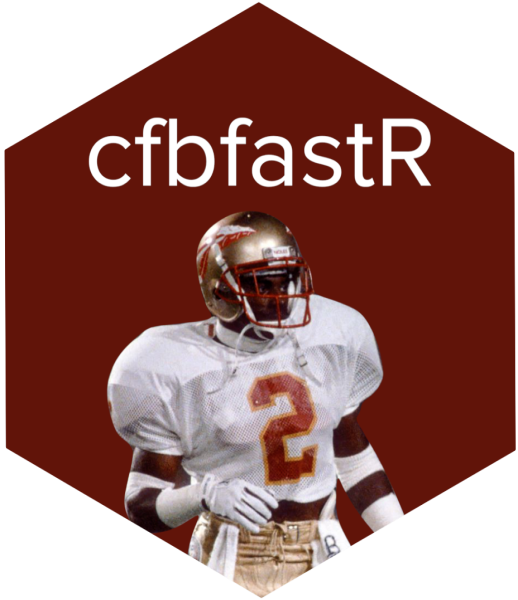
\includegraphics[width=0.1\textwidth]{./figures/cfbfastR.png}
    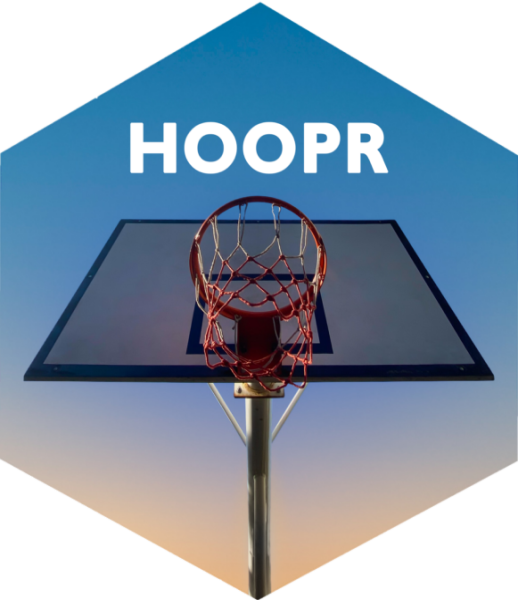
\includegraphics[width=0.1\textwidth]{./figures/hoopR.png}
    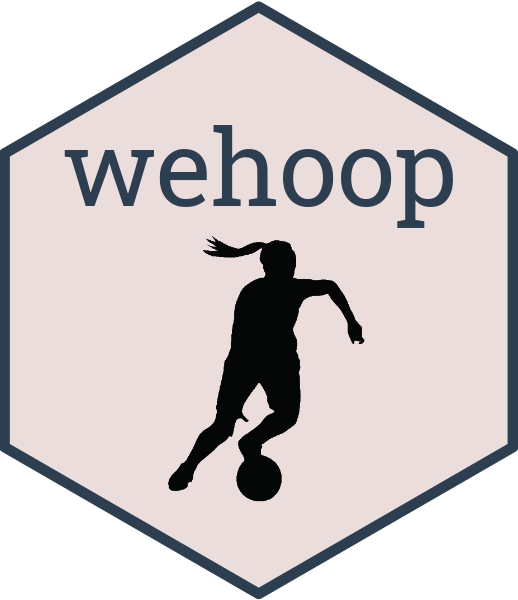
\includegraphics[width=0.1\textwidth]{./figures/wehoop.png}
    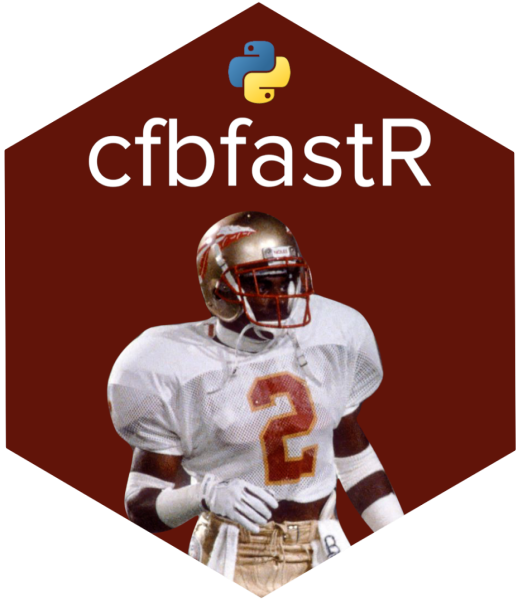
\includegraphics[width=0.1\textwidth]{./figures/cfbfastR-py.png}
    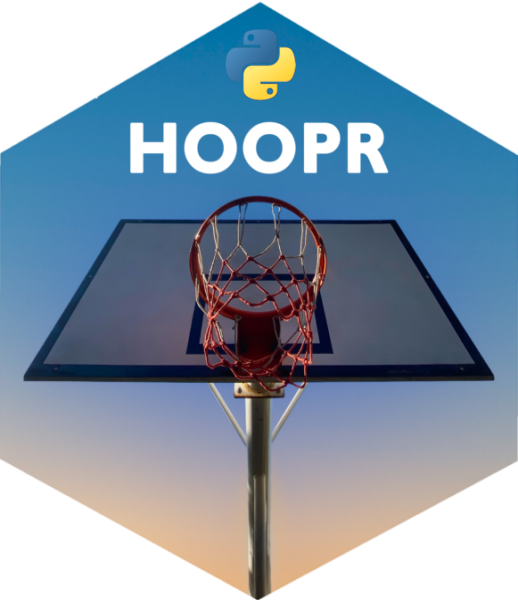
\includegraphics[width=0.1\textwidth]{./figures/hoopR-py.png}
    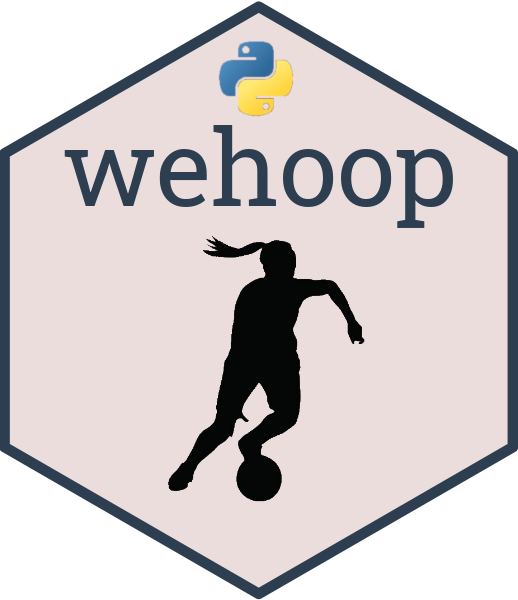
\includegraphics[width=0.1\textwidth]{./figures/wehoop-py.png}
    \label{fig:sdvR}
\end{figure} 
\newpage
\section{References}
\printbibliography[title={\hspace{5pt}\vspace{-10pt}}]


\end{document}
